\documentclass[10pt]{article}\usepackage[margin=.65in]{geometry}\usepackage[T1]{fontenc}\usepackage{graphicx}\setlength{\parindent}{0pt}\setlength{\parskip}{7pt}\sloppy\begin{document}{\large Source-ordered affine addition}\par 14 main declarations and 9 fixed controls compiled, with 23 separate named axiom readbacks. This packet archives completed producer evidence; independent review is pending.\par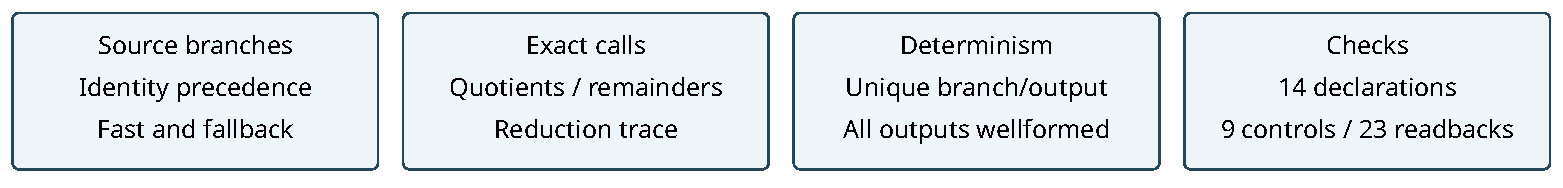
\includegraphics[width=\linewidth]{diagram.pdf}\par Construction. The source-ordered relation retains identity precedence, actual degree/norm/slope guards, successful fast quotient/remainder and constructor equations, and the fallback extended-gcd, exact-division and reduction traces. Output validity is not a premise of the execution relation. The construction proves total existence, unique branch and output, and wellformedness of every modeled execution. A general monic-list leading-word lemma connects normalized polynomial outputs to actual stored construction.

Assumptions and boundary. The domain is prime 2$<$p$<$2\textasciicircum{}31, canonical degree-five polynomial coefficients and wellformed stored inputs. The native correspondence covers n=1 with no tables. Canonical input slots remain an explicit premise. Identity returns retain original padding. The classifier represents branch outcomes, not operation scheduling or cost. It does not establish divisor-class addition or the quadratic-extension implementation.

Evidence. All successful receipts report unchanged bound inputs. The false theorem was rejected with exit one. Named readbacks contain only permitted foundational axioms. Exact sources, source snapshots, commands and failed attempts are under producer. Compiler and dependency caches were reused and hash-bound; no independent binary rechecker or transient-edit exclusion is claimed.

Retained failures and next work. One failed control attempt is retained. The requested separate corollary connecting dispatch outputs to the new stored-validity test was not created before the agent usage limit; it is pending, as is independent source-fidelity review.

Sources. The immutable native three\_leads.rs snapshot and dependency inventories are retained in producer, alongside the original detailed report. This composes existing source and polynomial proofs and makes no new-method claim. The graph shows proof structure because there are no comparative measurements. No scientific trajectory, cost ratio, runtime admission or campaign limit changed.
\end{document}